\begin{frame}{Recap From Previous Lecture}
    \begin{enumerate}
        \item Difference between Probability Mass Function (PMF) and Probability Density Function (PDF)
        \item Can a PMF ($f_X(x)$) take values larger than 1?\\(i.e. $f_X(x)>1$)
        \item Can a PDF ($f(x)$) take values larger than 1?\\(i.e. $f(x)>1$)
        \item Is expected value the same as mean?
    \end{enumerate}
\end{frame}

\section{Probability}

\begin{frame}{Complementary Events}

    The probability of all possible outcomes in an experiment is 1. \\
    If $\bar{A}$ is a complement event to $A$ then
    \begin{equation}
    P(\bar{A}) = 1 - P(A)
    \end{equation}

    \begin{example}
    \medskip
    \begin{columns}
        \begin{column}{0.65\textwidth}
            
            When tossing a fair coin the probability of getting ``head" (H) is related with the probability of getting ``tail" (T):
            \medskip
            
            $P(H) = 1 - P(T) = 1 - 0.5 = 0.5$
        \end{column}
        \begin{column}{0.25\textwidth}
            \includegraphics[width=0.75\textwidth]{gfx/web/coin}
        \end{column}
    \end{columns}
    \end{example}

\end{frame}

\begin{frame}{Independent Events}

    If events A and B are \emph{independent} then the joint probability is
    
    \begin{equation}
        P(A\text{ and }B) = P(A \cap B) = P(A)P(B)
    \end{equation}
    
    
    \begin{example}
        \medskip
        \begin{columns}
            \begin{column}{0.65\textwidth}
                What is the probability of getting an outcome (6, 6) in rolling a six-sided die twice?
            \end{column}
            \begin{column}{0.25\textwidth}
                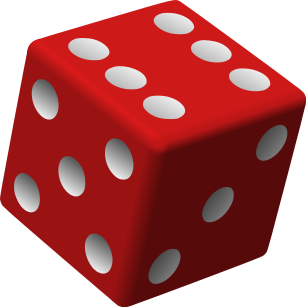
\includegraphics[width=0.5\textwidth]{gfx/web/die}
            \end{column}
        \end{columns}
    \end{example}
    \medskip
    \begin{shownto}{teacher}
        \pause
        $P(6 \cap 6) = P(6)P(6) = \frac{1}{6} \times \frac{1}{6} = \frac{1}{36}$
    \end{shownto}

\end{frame}

\begin{frame}{Mutually Exclusive Events}

    If events A and B are \emph{mutually exclusive} (\emph{disjoint}) then the probability of \textbf{both} occurring is
    \begin{equation}
    P(A\text{ and }B) = P(A \cap B) = 0
    \end{equation}
    
    However, the probability of \textbf{either} occurring is
    \begin{equation}
    \begin{split}
    P(A\text{ or }B) & = P(A \cup B) = \\
    & = P(A) + P(B) - P(A \cap B) = \\
    & = P(A) + P(B) - 0 = \\
    & = P(A) + P(B)
    \end{split}
    \end{equation}
    
\end{frame}

\begin{frame}{Mutually Exclusive Events}

    \begin{example}
    \medskip
    \begin{columns}
        \begin{column}{0.65\textwidth}
            What is the probability of getting an outcome 1 or 3 in rolling a six-sided die?
        \end{column}
        \begin{column}{0.25\textwidth}
            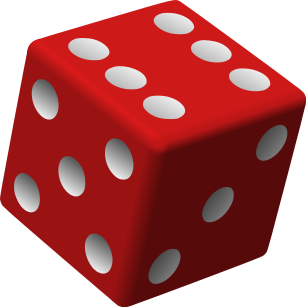
\includegraphics[width=0.5\textwidth]{gfx/web/die}
        \end{column}
    \end{columns}
    \end{example}
    \medskip
    \begin{shownto}{teacher}
        \pause
        \begin{equation*}
        P(1\text{ or }3) = P(\{1, 3\}) = P(1 \cup 3) = P(1) + P(3) = \frac{1}{6} + \frac{1}{6} = \frac{1}{3}
        \end{equation*}
    \end{shownto}
    
    \pause
    \begin{example}
        \medskip
        \begin{columns}
            \begin{column}{0.65\textwidth}
                What is the probability of getting a sum of 11 in rolling two six-sided dice?
            \end{column}
            \begin{column}{0.25\textwidth}
                \includegraphics[width=\textwidth]{gfx/web/dice}
            \end{column}
        \end{columns}
    \end{example}
    \medskip
    \begin{shownto}{teacher}
        \pause
        \begin{equation*}
        P((6 \cap 5) \cup (5 \cap 6)) = P((6, 5) \cup (5, 6)) = \frac{1}{36} + \frac{1}{36} = \frac{1}{18}
        \end{equation*}
    \end{shownto}


\end{frame}


\begin{frame}{Not Mutually Exclusive Events}
    If two events are not mutually exclusive then $P(A \cap B) \neq 0$ and
    \begin{equation}
    P(A\text{ or }B) = P(A \cup B) = P(A) + P(B) - P(A \cap B)
    \end{equation}
    
    \begin{figure}
        
\includegraphics[width=0.4\linewidth]{gfx/sets_AB}
    \end{figure}
\end{frame}

\begin{frame}[t]{Not Mutually Exclusive Events}
    \only<1-2>{
        \begin{example}
        \medskip
        For example, when drawing a single card at random from a regular deck of cards, the chance of getting a heart or a face card (J, Q, K) (or one that is both) is \showto{teacher}{
            \only<1>{...}
            \only<2>{
                $\frac{13}{52} + \frac{12}{52} - \frac{3}{52} = \frac{11}{26}$.
            }
        }
        \showto{students}{...}
        \end{example}
    }
    \only<1>{
        \includegraphics[width=\textwidth]{gfx/web/cards}
        {\tiny Source: \url{https://en.wikipedia.org/wiki/Standard_52-card_deck}}
    }
    \only<2>{
        \includegraphics[width=\textwidth]{gfx/overlapping_probabilities}
    }
\end{frame}

\begin{frame}{Not Mutually Exclusive Events}

    \begin{example}
        \medskip
        When drawing a single card from a regular deck of cards, what is the probability of getting a spade OR an ace?
    \end{example}
    \begin{shownto}{teacher}
        \pause
        $P(S \cup A) = \frac{13}{52} + \frac{4}{52} - \frac{1}{52} = \frac{16}{52} $
        \pause
    \end{shownto}
    
    \begin{example}
        \medskip
        When drawing a single card from a regular deck of cards, what is the probability of getting a spade OR a diamond OR an ace?
    \end{example}
    \begin{shownto}{teacher}
        \pause
        \begin{align*}
        P(S \cup D \cup A) &= \frac{13}{52} + \frac{13}{52} + \frac{4}{52} - \frac{1}{52} - \frac{1}{52} - 0 - 0 = \frac{28}{52}\\
        P((S \cup D) \cup A ) &= P(S \cup D) + P(A) - P((S \cup D) \cap A) =\\
                             &= \frac{26}{52} + \frac{4}{52} - \frac{2}{52} = \frac{28}{52}
        \end{align*}
    \end{shownto}

\end{frame}

\begin{frame}{Joint Probability of Three Sets}
    \begin{figure}
        
\includegraphics[width=0.4\linewidth]{gfx/sets_ABC}
    \end{figure}
    \begin{align}
    \begin{split}
    P(A \cup B \cup C) &= P(A) + P(B) + P(C)\\
                       &\qquad - P(A \cap B) - P(A \cap C) - P(C \cap B)\\
                       &\qquad + P(A \cap B \cap C)
    \end{split}
    \end{align}
\end{frame}

\begin{frame}{Conditional Probability}

    \begin{figure}
        
\includegraphics[width=0.3\linewidth]{gfx/sets_AB}
    \end{figure}
    If $A$ depends on $B$ then the probability of $A$ given $B$ is
    \begin{equation}
    P(A|B) = \frac{P(A \cap B)}{P(B)}
    \end{equation}
  
    Note that if $A$ and $B$ are independent then  
    \begin{equation}
    P(A|B) = \frac{P(A) P(B)}{P(B)} = P(A),
    \end{equation}
    confirming that $B$ has no effect on $A$.

\end{frame}

\begin{frame}{Conditional Probability}
    \medskip
    \begin{example}
        \medskip {\small
        Meteorological observations for wind speed $w$ and atmospheric pressure $p_{atm}$ were taken during 1000 days (one measurement per day). Let $A$ stand for $ w < 6$ m/s, $\bar{A}$ for $w \geq$ 6 m/s, $B$ for $p_{atm} < 1000$ hPa, and $\bar{B}$ for $p_{atm} \geq 1000$ hPa. The measurements are summarized in the following frequency table:
        \vspace{-5pt}
        \begin{table}
            \begin{tabular}{c | c c c}
                            & $A$   & $\bar{A}$     & Sum \\ \hline
                $B$         & 400   & 100           & 500 \\
                $\bar{B}$   & 200   & 300           & 500 \\
                Sum         & 600   & 400           & 1000 \\
            \end{tabular}
        \end{table}
        Using conditional probability, prove that $w$ depends on $p_{atm}$.}
        
        {\tiny
        Hint: Show that $P(A) \neq P(A|B)$.
        }
    \end{example}
\end{frame}

\begin{frame}{The Law of Total Probability}
    \begin{figure}
        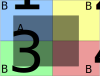
\includegraphics[width=0.3\linewidth]{gfx/total_probability_boxes}
    \end{figure}
    The total (marginal) probability can be calculated from all possible conditional probabilities:
    \begin{equation}
    P(A) = \sum_{i} P(A \cap B_i) = \sum_{i} P(A|B_i) P(B_i) \label{eq:marginal_probability}
    \end{equation}

    If $B$ has only two possible outcomes:
    \begin{equation*}
    P(A) = P(A|B) P(B) + P(A|\bar{B}) P(\bar{B})
    \end{equation*}
\end{frame}

\begin{frame}{The Law of Total Probability: Tabular Explanation}
   
    Relative frequency table:
    \begin{table}
        \begin{tabular}{c | c c c}
                       & $A$  & $\bar{A}$ & Sum \\ \hline
            $B$        & 0.4  & 0.1       & 0.5 \\
            $\bar{B}$  & 0.2  & 0.3       & 0.5 \\
            Sum        & 0.6  & 0.4       & 1.0 \\
        \end{tabular}
    \end{table}
    Show that $P(A) = P(A|B)P(B) + P(A|\bar{B})P(\bar{B})$.
\end{frame}

\begin{frame}{The Law of Total Probability: Graphical Explanation}
    \begin{columns}
        \begin{column}{0.6\textwidth}
            {\small
            \begin{align*}
            P(A) &= \frac{(a+b)c}{(a+b)(c+d)} = \frac{c}{c+d} \\
            P(A|F) &= \frac{bc}{bc+de} \\
            P(F) &= \frac{bc+de}{(a+b)(c+d)} \\
            P(A|\bar{F}) &= \frac{ac}{ac+df} \\
            P(\bar{F}) &= \frac{ac+df}{(a+b)(c+d)}
            \end{align*}
            }
        \end{column}
        \begin{column}{0.4\textwidth}
            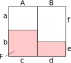
\includegraphics[width=\linewidth]{gfx/total_probability}
        \end{column}
    \end{columns}
    {\small
    \begin{align*}
    P(A)    &= P(A|F)P(F) + P(A|\bar{F})P(\bar{F}) = \\
            &= \frac{bc}{(a+b)(c+d)} + \frac{ac}{(a+b)(c+d)} = \\
            &= \frac{ac+bc}{(a+b)(c+d)} = \frac{(a+b)c}{(a+b)(c+d)} = \frac{c}{c+d}
    \end{align*}}
\end{frame}

\begin{frame}{Bayes' Theorem: Exemplary Problem}
    %Example based on: \url{https://www.youtube.com/watch?v=R13BD8qKeTg}
    \begin{example}
        \medskip    
        A person has been tested positive for a rare disease. The test correctly identifies 99\% of people having the disease, however 1\% of people not having the disease is also falsely tested as positive. It is estimated that the disease is present in 0.1\% of the population.
        
        What is the probability that the person has the disease?
        
        $P(+|D) = 0.99$\\
        $P(+|H) = 0.01$\\
        $P(D) = 0.001$\\
        $P(D|+) =$ ?
        
        Discuss in groups.
    \end{example}
\end{frame}

\begin{frame}{Bayes' Theorem: Exemplary Problem}
    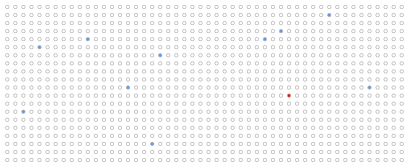
\includegraphics[width=\linewidth]{gfx/dots_disease}
\end{frame}

\begin{frame}{Bayes' Theorem}
    Bayes' theorem describes the probability of an event, based on prior knowledge of conditions that might be related to the event. Mathematically, it can be described as follows:
    \begin{equation}
    P(A|B) = \frac{P(B|A)P(A)}{P(B)} = \frac{P(B|A) P(A)}{\sum_{i} P(B|A_i)P(A_i)}
    \end{equation}
    
    where $A$ and $B$ are events and $P(B) \neq 0$.
    
    \begin{itemize}
        \item $P(A|B)$ -- the likehood of A given that B is true
        \item $P(B|A)$ -- the likehood of B given that A is true
        \item $P(A)$ and $P(B)$ -- marginal probabilities $\rightarrow$ Eq.~(\ref{eq:marginal_probability})
    \end{itemize}
\end{frame}

\begin{shownto}{teacher}
\begin{frame}{Disease Example Solution}

    \begin{align*}
    P(D|+)  &= \frac{P(+|D)P(D)}{P(+)} = \\
            &= \frac{P(+|D)P(D)}{P(+|D)P(D) + P(+|H)P(H)} = \\
            &= \frac{0.99 \times 0.001}{0.99 \times 0.001 + 0.01 \times 0.999}= \\
            &= 0.09 =\\
            &= 9\% \\
    \end{align*}

\end{frame}
\end{shownto}

\begin{frame}{Bayes' Theorem}
    \begin{example}
        \medskip
        {\small
        There are two factories (A and B) manufacturing the same type of a device and both releasing 5000 devices per year to the market. 2 out of 100 devices manufactured in factory A are faulty. 5 out of 1000 devices manufactured in factory B are faulty. If you a buy a faulty device, what is the probability it was produced in the factory A?}
    \end{example}
    \medskip
    \begin{columns}
        \begin{column}{0.35\textwidth}
            \begin{tabular}{c | c | c | c}
                & $A$   & $B$   & $\sum$ \\ \hline
                $F$       & 2     & 5     & 7 \\ \hline
                $\bar{F}$ & 98    & 995   & 1093 \\ \hline
                $\sum$    & 100   & 1000  & 1100 \\
            \end{tabular}  
        \end{column}
        
        \begin{column}{0.6\textwidth}
            \begin{shownto}{teacher}
            \pause
            {\small
            \begin{align*}
            P(A|F) &= \frac{P(F|A) P(A)}{P(F)} =\\
                   &= \frac{P(F|A) P(A)}{P(F \cap A) + P(F \cap B)} =\\
                   &= \frac{P(F|A) P(A)}{P(F|A) P(A) + P(F|B) P(B)} =\\
                   &= \frac{\frac{2}{100} \times \frac{1}{2}}{\frac{2}{100}\times\frac{1}{2} + \frac{5}{1000}\times\frac{1}{2}} = \frac{4}{5}\\
            \end{align*}
            }
            \end{shownto}
        \end{column}
    \end{columns}
\end{frame}

\begin{frame}{Probability: Summary}
    \begin{align*}
    P(A) & \in [0, 1] \\
    P(\bar{A}) &= 1 - P(A) \\[3ex]
    P(A \cup B) &= P(A) + P(B) - P(A \cap B) \\
    P(A \cup B) &= P(A) + P(B) \qquad \leftarrow \text{if A and B mut. exclusive} \\[3ex]
    P(A \cap B) &= P(A|B)P(B) = P(B|A)P(A) \\
    P(A \cap B) &= P(A)P(B) \qquad \leftarrow \text{if A and B independent} \\[3ex]
    P(A|B) &= \frac{P(A \cap B)}{P(B)} = \frac{P(B|A)P(A)}{P(B)} \\
    \end{align*}
\end{frame}

\begin{frame}{Exercises}
    \begin{example}
        \medskip
        Assume that 5\% of students (group 1) can answer to all exam questions, 30\% (group 2) can answer 70\% questions, 40\% (group 3) can answer 60\% questions, 25\% (group 4) can answer 50\% questions.
        \begin{enumerate}
            \item What is the probability that a randomly selected student can answer a question?
            \item What is the probability that a student who correctly answered a question belongs to the group no. 2?
        \end{enumerate}
    \end{example}
\end{frame}

\begin{shownto}{teacher}
    \begin{frame}{Exercises}
        1. What is the probability that a randomly selected student can answer a question?
        \medskip
        
        \begin{align*}
        P(A)    &= P(G_1, A) + P(G_2, A) + P(G_3, A) + P(G_4, A) =\\
                &= \sum_{i=1}^{4}P(G_i)P(A|G_i) =\\
                &= 0.05 \times 1 + 0.3 \times 0.7 + 0.4 \times 0.6 + 0.25 \times 0.5 =\\
                &= 0.625
        \end{align*}
    \end{frame}
    
    \begin{frame}{Exercises}
        2. What is the probability that a student who correctly answered a question belongs to the group no. 2?
        \medskip
        
        \begin{align*}
        P(G_2|A)    &= \frac{P(G_2, A)}{P(A)} = \frac{0.3 \times 0.7}{0.625} = 0.336
        \end{align*}
    \end{frame}
\end{shownto}

\begin{frame}{Exercises}
    \begin{example}
        \medskip
        Within 200 sensors 8 are faulty. We have to randomly select 3 sensors. What is the probability that all of them will be faulty?
        \begin{shownto}{teacher}
            \medskip
            \pause
            \begin{equation*}
            P(F) = \frac{8}{200} \times \frac{7}{199} \times \frac{6}{198} = 0.000043
            \end{equation*}
        \end{shownto}

    \end{example}
\end{frame}

\begin{frame}{Exercises}
    \begin{example}
        \medskip
        The numbers $1, 2, 3, ..., n$ are put in a random sequence.
        \begin{enumerate}
            \item What is the probability that the numbers 1, 2 are put next to each other and exactly in this order?
            \item What is the probability that the numbers 1, 2, 3 are put next to each other and exactly in this order?
        \end{enumerate}
    \end{example}
\end{frame}

\begin{shownto}{teacher}
    \begin{frame}{Exercises}
        1. What is the probability that the numbers 1, 2 are put next to each other and exactly in this order?
        \medskip
        
        \begin{itemize}
            \item Number of possible positions of $\{1,2\}$ within an $n$-element sequence is $(n-1)$.
            \item Number of possible permutations of an $(n-2)$-element sequence is $(n-2)!$.
            \item Number of possible permutations of an $n$-element sequence is $n!$.
            \item Final answer: $\frac{(n-1)(n-2)!}{n!} = \frac{(n-1)!}{n!} = \frac{1}{n}$.
        \end{itemize}
    \end{frame}

    \begin{frame}{Exercises}
        2. What is the probability that the numbers 1, 2, 3 are put next to each other and exactly in this order?
        \medskip
        
        \begin{itemize}
            \item Number of possible positions of $\{1,2,3\}$ within an $n$-element sequence is $(n-2)$.
            \item Number of possible permutations of an $(n-3)$-element sequence is $(n-3)!$.
            \item Number of possible permutations of an $n$-element sequence is $n!$.
            \item Final answer: $\frac{(n-2)(n-3)!}{n!} = \frac{(n-2)!}{n!} = \frac{1}{n(n-1)}$.
        \end{itemize}
    \end{frame}

\end{shownto}

\begin{frame}{Hands-on Training: R}
    \begin{itemize}
        \item Calculating the mean, variance, standard deviation, covariance
        \item Data frames
        \item R Base Graphics
    \end{itemize}
\end{frame}

\begin{frame}{Homework}
    Read the following chapters of ``R for Data Science":
    \begin{itemize}
        \item \url{http://r4ds.had.co.nz/introduction.html}
        \item \url{http://r4ds.had.co.nz/explore-intro.html}
        \item \url{http://r4ds.had.co.nz/data-visualisation.html}
    \end{itemize}

    Install ``tidyverse", as described in Section 1.4.3.
\end{frame}